\section{Analizator sygnałów logicznych - test zaprojektowanego systemu}
    W celu przetestowania układu należy wygenerować odpowiednio duży wektor testowy,
    pozwalający na rzetelne sprawdzenie wszystkich możliwych kombinacji.
    Jednocześnie wektor ten powinien był w miarę możliwości prosty do sprawdzenia.
    Dlatego też jako wektor testowy wykorzystano licznik binarny, który z każdym stanem powinien rosnąć o dokładnie \textit{,,1''}.

    Poniżej przedstawiono zdjęcie aplikacji wyświetlającej 512 próbek odebranych za pomocą analizatora.
    \begin{figure}[!ht]
        \centering
        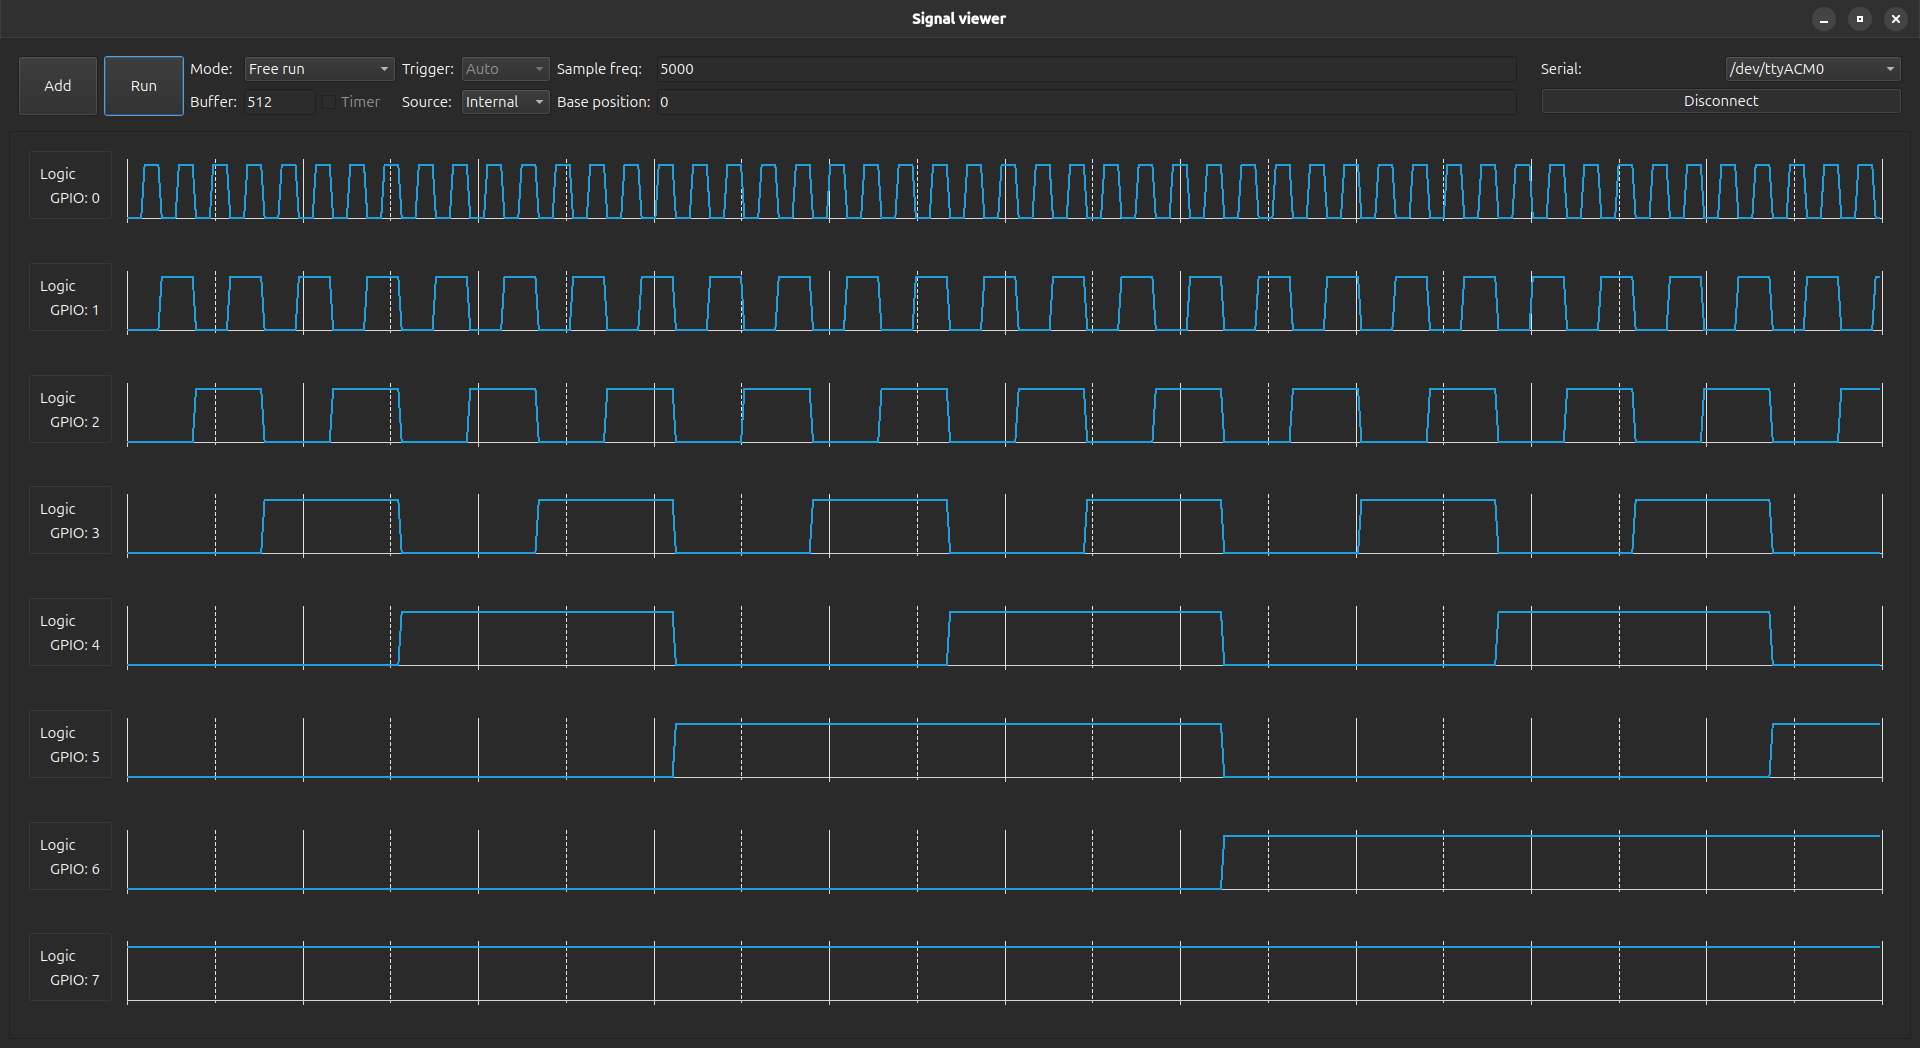
\includegraphics[width=0.8\textwidth]{test_1khz.png}
        \caption{Zdjęcie aplikacji - pomiar testowy, częstotliwość sygnału 1kHz}
    \end{figure}

    Odczytana częstotliwość na podstawie ilości próbek: $f_{read} = 1kHz$, co odpowiada zadanej częstotliwości wejściowej.

    Analizowanie wyższych częstotliwości w aktualnej wersji programu graficznego jest niemożliwe, ze względu na bug w kodzie aplikacji, która nie zmienia ustawień analizatora.
    Natomiast przed rozpoczęciem pracy z aplikacją graficzną, analizator został przetestowany, sygnał cyfrowym przedstawionym poniżej:
    \begin{figure}[!ht]
        \centering
        \begin{tikzpicture}
            \draw
                (0, 0) 
                    --++ (1, 0) --++(0, 1) --++(1, 0) --++ (0, -1)
                    --++ (1, 0) --++(0, 1) --++(1, 0) --++ (0, -1)
                    --++ (1, 0) --++(0, 1) --++(1, 0) --++ (0, -1)
                    --++ (1, 0) --++(0, 1) --++(1, 0) --++ (0, -1)

                    --++(4, 0)
                    --++ (1, 0) --++(0, 1) --++(1, 0) --++ (0, -1)
            ;

            \draw [Stealth-Stealth] (2, 1.5) -- node[above]{50MHz} (4, 1.5);
            \draw [Stealth-Stealth] (1, -0.5) -- node[above]{1kHz} (13, -0.5);
        \end{tikzpicture}
    \end{figure}

    Dla takiego sygnału udało się odebrać odebrać licznik binarny, którego złożenie przedstawiono na wykresie \ref{fig:sampling}.
    \newpage
    \begin{figure}[!ht]
        \centering
        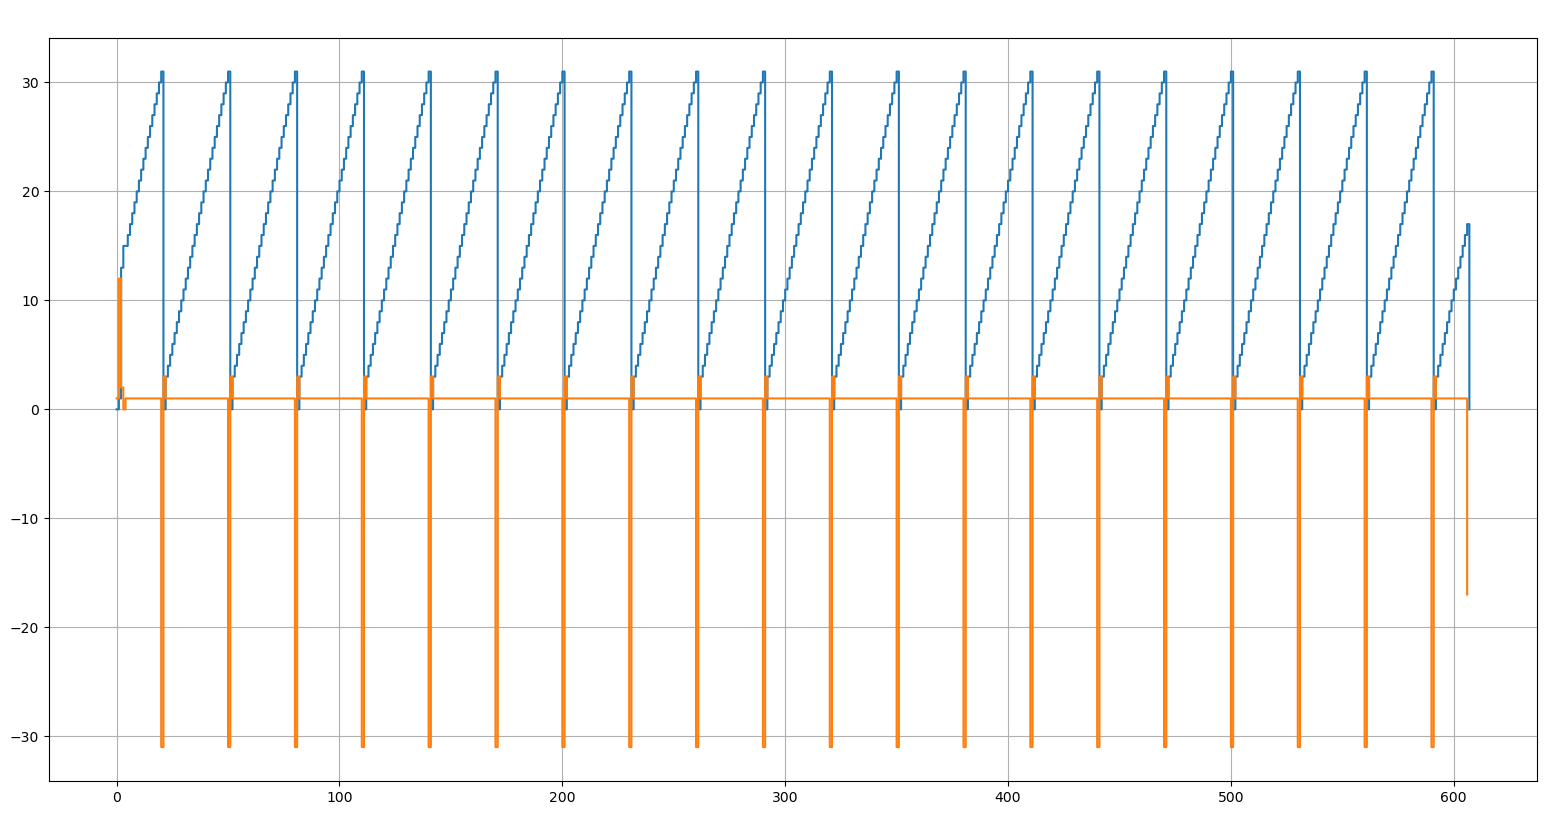
\includegraphics[width=0.8\textwidth]{Sampling.png}
        \caption{Wykres przebiegu odebranego dla sygnału o maksymalnej częstotliwości $50MHz$}
        \label{fig:sampling}
    \end{figure}
    \begin{itemize}
        \item na pomarańczowo oznaczono różnicę między aktualną a poprzednią próbką,
        \item niebieskim zaprezentowano odebraną próbkę.
    \end{itemize}

    \subsection{Zaobserwowane problemy z działaniem analizatora}
        Największym problemy działania analizatora jest utrata próbek podczas analizy bardzo szybkich sygnałów w trybie \textit{Free Run}.
        Podczas pracy kołowej kołowej analizator nie jest w stanie wysyłać próbek tak szybko jak układ PIO i DMA zapisują nowe dane.
        Rozwiązaniem tego problemu jest nie wykorzystywanie tego trybu do analizy ciągłych bardzo szybkich sygnałów.


    